\documentclass[12pt,titlepage,landscape,a4paper]{article}

%QUELQUES PACKAGES PLUS OU MOINS UTILES
\special{landscape}
\usepackage[T1]{fontenc}
\usepackage[utf8]{inputenc}
\usepackage[english]{babel}
\usepackage{amsfonts, amsmath, amssymb, amsthm, mathtools}
\usepackage{aeguill}
\usepackage{graphics, graphicx}
\usepackage{xcolor}
\usepackage{geometry}
\usepackage{paralist}
\usepackage{multido,ifthen}
\usepackage{tikz}
\usetikzlibrary{trees, decorations, decorations.markings, shapes, arrows, matrix, calc, fit, intersections, patterns, angles, snakes}
\usepackage[external]{forest}
\usepackage{hyperref}
\hypersetup{colorlinks=true, citecolor=blue, linkcolor=blue, urlcolor=blue}
\usepackage{movie15}
\usepackage[abs]{overpic}
\usepackage{xargs}
\usepackage{extarrows}
\usepackage{shuffle}
\usepackage{multicol}
\usepackage{etoolbox}
\usepackage{dsfont}
\usepackage{pifont}
\usepackage{array, blkarray}
\usepackage{multicol, multirow}
\usepackage{ulem}
\usepackage{xifthen}

% ZONE DE TEXTE ET POLICE
\setlength{\topmargin}{-2.8cm}
\setlength{\textheight}{19cm}
\setlength{\oddsidemargin}{-1cm}
\setlength{\textwidth}{26.8cm}
\newcommand{\textenormal}{\fontsize{22}{28}\selectfont}
\newcommand{\textemoyen}{\fontsize{23}{27}\selectfont}
\newcommand{\textegrand}{\fontsize{55}{48}\selectfont}

% COMMANDE DE NOUVELLE PAGE
\newenvironment{slide}[1]
{
\newpage
\begin{center}
{\blue \textemoyen \uppercase{#1}}\\
\end{center}
\vspace{-1cm}
\rule{\textwidth}{0.5 pt}\\
\vspace{-.8cm}
}
{\vspace*{-3cm}}

% COMMANDE DE PARTIE
%\newcounter{partie}
%\setcounter{partie}{1}
%\newcommand{\thePartie}{Part \arabic{partie}}
\newcommand{\partie}[1]
{
\newpage
\vspace*{0pt plus 1 fill}
\begin{center}
%\thePartie \\[-.75cm]
\rule{.9\textwidth}{0.5 pt} \\[.5cm]
\fontsize{30}{30}\selectfont {\blue \uppercase{#1}} \\[-.35cm]
\rule{.9\textwidth}{0.5 pt} \\
\end{center}
\vspace*{0pt plus 1.2 fill}
%\addtocounter{partie}{1}
}

% COMMANDE D'EXPOSE
\newcommand{\expose}[2]
{
\newpage
\vspace*{0pt plus 1 fill}
\begin{center}
%\thePartie \\[-.75cm]
\rule{.8\textwidth}{0.5 pt} \\[.5cm]
\fontsize{35}{35}\selectfont {\red\uppercase{#1}} \\[-.35cm]
\rule{.8\textwidth}{0.5 pt} \\
\vspace{1cm}
\textemoyen #2
\end{center}
\vspace*{0pt plus 1.2 fill}
%\addtocounter{partie}{1}
}

% COMMANDE POUR LES BOITES
% centre
\newcommand{\cboite}[1]
{
\vspace*{.5cm}
\fcolorbox{blue}{grisclair}{
\begin{minipage}{.97\linewidth}
\vspace*{.3cm}
\begin{center} #1 \end{center}
\vspace*{-.1cm}
\end{minipage}
}
}
% alignement gauche
\newcommand{\gboite}[1]
{
\vspace*{.5cm}
\fcolorbox{blue}{grisclair}{
\begin{minipage}{.97\linewidth}
\vspace*{.3cm}
#1
\vspace{.3cm}
\end{minipage}
}
}

\newcommand{\chapitre}[1]{{\blue \fontsize{23}{25}\selectfont {Chap\,#1}}}

% AUTRES COMMANDES
% quelques couleurs manquantes
\newcommand{\orange}{\color{orange}} % couleur orange
\newcommand{\green}{\color{green}} % couleur verte
\newcommand{\violet}{\color{violet}} % couleur violet
\newcommand{\blue}{\color{blue}} % couleur bleu
\newcommand{\red}{\color{red}} % couleur rouge
\definecolor{violet}{rgb}{.5,.1,.9}
\definecolor{orange}{rgb}{.94,.57,0}
\definecolor{green}{rgb}{0.2,0.6,0.2}
\definecolor{grisclair}{gray}{1}
\definecolor{grisfonce}{gray}{.1}
\definecolor{bblue}{rgb}{.8,.8,1}
% maths
\newcommand{\set}[2]{\left\{ #1 \;\middle|\; #2 \right\}} % ensemble
\newcommand{\bigset}[2]{\big\{ #1 \;\big|\; #2 \big\}} % ensemble
\newcommand{\biggset}[2]{\bigg\{ #1 \;\bigg|\; #2 \bigg\}} % ensemble
\newcommand{\setangle}[2]{\left\langle #1 \;\middle|\; #2 \right\rangle} % ensemble
\newcommand{\dotprod}[2]{\left\langle\; #1 \;\middle|\; #2 \;\right\rangle} % produit scalaire
\newcommand{\ssm}{\smallsetminus} % small set minus
\newcommand{\symdif}{\triangle} % symmetric difference
\newcommand{\eqdef}{\mbox{\,\raisebox{0.3ex}{\normalsize\ensuremath{\mathrm:}}\ensuremath{=}\,}} % :=
\newcommand{\defeq}{\mbox{~\ensuremath{=}\raisebox{0.3ex}{\normalsize\ensuremath{\mathrm:}} }} % =:
\newcommand{\Fracfloor}[2]{\left\lfloor \frac{#1}{#2} \right\rfloor} % floor of a fraction
\newcommand{\one}{1\!\!1} % one bold
\DeclareMathOperator{\conv}{conv} % enveloppe convexe
\DeclareMathOperator{\cone}{cone} % cone engendre
\DeclareMathOperator{\vol}{vol} % volume
\newcommand{\C}{\mathbb{C}} % complexes
\newcommand{\R}{\mathbb{R}} % reels
\newcommand{\Z}{\mathbb{Z}} % entiers
\newcommand{\N}{\mathbb{N}} % naturels
\newcommand{\I}{\mathbb{I}} % set of integers
\newcommand{\K}{\mathbb{K}} % field
\newcommand{\fS}{\mathfrak{S}} % symmetric group
\newcommand{\cA}{\mathcal{A}} % algebra
\newcommand{\cF}{\mathcal{F}} % flip graph
\newcommand{\cN}{\mathcal{N}} % sorting network
\renewcommand{\b}[1]{\boldsymbol{#1}} % bold letters
\renewcommand{\c}[1]{\mathcal{#1}} % caligraphic letters
\newcommand{\f}[1]{\mathfrak{#1}} % frak letters
\newcommand{\bb}[1]{\mathbb{#1}} % bbold letters
% autres
\setlength{\parindent}{0pt} % aucune indentation dans tout le document
\graphicspath{{figures/}{figures/nodes/}} % les repertoires ou se trouvent les figures
\newcommand{\papier}[1]{{\violet\fontsize{15}{20}\selectfont #1}} % citation papier
\newcommand{\theo}[2]{\gboite{{\blue \fontsize{18}{25}\selectfont #1.} #2}}
\newcommand{\HUGE}[1]{{\fontsize{35}{33}\selectfont #1}}
\newcommand{\esperluette}{ \\ --- \& --- \\ } % esperluette stylisée nouvelle ligne
\DeclareRobustCommand{\verylongrightarrow}{\joinrel\relbar\joinrel\relbar\joinrel\relbar\joinrel\relbar\joinrel\relbar\joinrel\rightarrow}
\renewcommand{\emph}[1]{\uline{#1}}

% specific wiggly
\newcommand{\polytope}[1]{\mathds{#1}} % font polytope
\newcommand{\wigglyComplex}{\mathrm{WC}} % wiggly complex
\newcommand{\wigglyFlipGraph}{\mathrm{WFG}} % wiggly flip graph
\newcommand{\wigglyIncreasingFlipGraph}{\mathrm{WIFG}} % wiggly increasing flip graph
\newcommand{\wigglyLattice}{\mathrm{WL}} % wiggly lattice
\newcommand{\wigglyFan}{\mathrm{WF}} % wiggly fan
\newcommand{\wigglyhedron}{\polytope{W}} % wigglyhedron
\newcommand{\Asso}{\polytope{A}\mathsf{sso}} % associahedron
\newcommand{\HH}{\mathbb{H}} % hyperplane
\newcommand{\HS}{\b{H}^\ge} % half-space

%%%%%%%%%%%%%%%%%%%%%%%%%%%%%%%%%%%%%%%%%%%%%%%%

\newcommand{\titre}{From permutahedra to associahedra, a walk through geometric and algebraic combinatorics}
\newcommand{\auteur}{Vincent Pilaud}

%%%%%%%%%%%%%%%%%%%%%%%%%%%%%%%%%%%%%%%%%%%%%%%%

\begin{document}

\fontshape{sf}\fontsize{22}{28}\selectfont % police par defaut
\sf
\pagestyle{empty} % bas de page par defaut

\vspace*{-1cm}
\begin{center}
{\blue \fontsize{60}{60}\selectfont
\uppercase{Wigglyhedra}

}

\vspace{.8cm}

A. BAPAT
(The Australian National University)

V. PILAUD
(Universitat de Barcelona)


\href{https://arxiv.org/abs/2407.11632}{\texttt{arxiv:2407.11632}}

\vspace{-.2cm}
\centerline{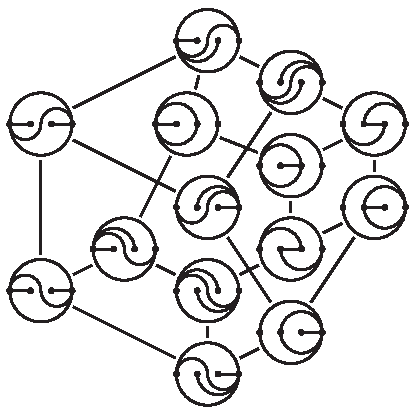
\includegraphics[scale=1.8]{wigglyFlipGraph}\quad\raisebox{.5cm}{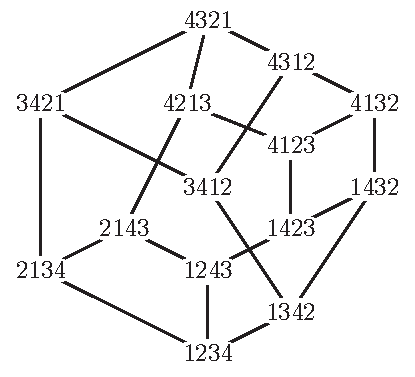
\includegraphics[scale=1.8]{wigglyLattice}}}

\vspace{.1cm}
DMG Seminar Berlin --- October 9, 2024

\vspace*{-.6cm}

\end{center}

%%%%%%%%%%%%%%%%%%%%%%%%%%%%%%%%%%%%%%%%%%%%%%%%%%%%%%

\partie{Triangulations \& associahedra}

%%%%%%%%%%%%%%%%%%%%%%%%%%%%%%%%%%%%%%%%%%%%%%%%%%%%%%

\begin{slide}{ASSOCIAHEDRON}

\gboite{
\emph{Associahedron} = polytope whose face lattice is isomorphic to the lattice of crossing-free sets of internal diagonals of a convex $(n+3)$-gon, ordered by reverse inclusion
}

\vspace{.2cm}
\centerline{\includegraphics[scale=3.1]{associahedron}}
\vspace*{-3.5cm}
\begin{tabular}{r@{ $\leftrightarrow$ }l}
vertices & triangulations \\
edges & flips \\
faces & dissections
\end{tabular}
\hfill
\begin{tabular}{r@{ $\leftrightarrow$ }l}
vertices & binary trees \\
edges & rotations \\
faces & Schr\"oder trees
\end{tabular}

\end{slide}

%%%%%%%%%%
%
%\begin{slide}{VARIOUS ASSOCIAHEDRA}
%
%\gboite{
%\emph{Associahedron} = polytope whose face lattice is isomorphic to the lattice of crossing-free sets of internal diagonals of a convex $(n+3)$-gon, ordered by reverse inclusion
%}
%
%\vspace{.5cm}
%\centerline{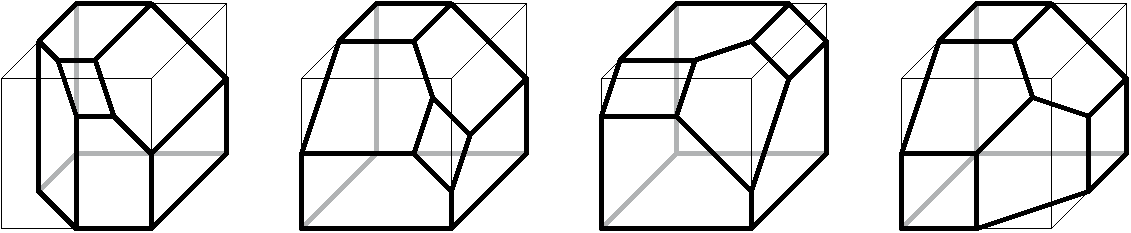
\includegraphics[width=\textwidth]{manyAssociahedra1}}
%\vspace{.5cm}
%\centerline{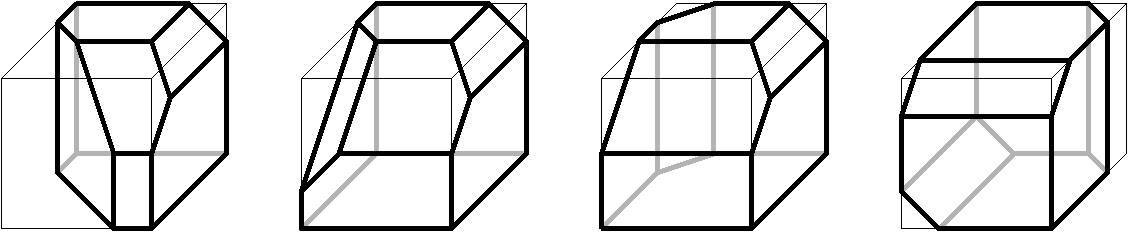
\includegraphics[width=\textwidth]{manyAssociahedra2}}
%
%\vspace{-.2cm}
%\hfill {\normalsize (Pictures by Ceballos-Santos-Ziegler)}
%
%\vspace{-.9cm}
%\papier{
%
%Tamari ('51) --- Stasheff ('63) --- Haimann ('84) --- Lee ('89) --- \hspace*{12.5cm} \\[.2cm]
%\dots --- Gel'fand-Kapranov-Zelevinski ('94) --- \dots --- Chapoton-Fomin-Zelevinsky ('02) --- \dots --- Loday ('04) --- \dots \hspace*{1.5cm} \\[.2cm]
%--- Ceballos-Santos-Ziegler ('11)
%
%}
%
%\end{slide}

%%%%%%%%%

\begin{slide}{THREE FAMILIES OF REALIZATIONS}

\vspace{-.25cm}
\hspace{-1.2cm}
\begin{tabular}{cc|ccc|cc}
\begin{minipage}[t]{8.5cm}
\begin{center}
{\blue SECONDARY} \\ {\blue POLYTOPE} \\[.5cm]
\end{center}
\vspace{-.2cm}
\centerline{\includegraphics[scale=1.5]{associahedron}}
\vspace{.1cm}
\papier{Gelfand--Kapranov--Zelevinsky ('94) \\ Billera--Filliman--Sturmfels ('90)

}
\vspace{8cm}
\end{minipage}
&&&
\begin{minipage}[t]{8.5cm}
\begin{center}
{\blue LODAY'S ASSOCIAHEDRON} \\[.5cm]
\end{center}
\vspace{-.2cm}
\centerline{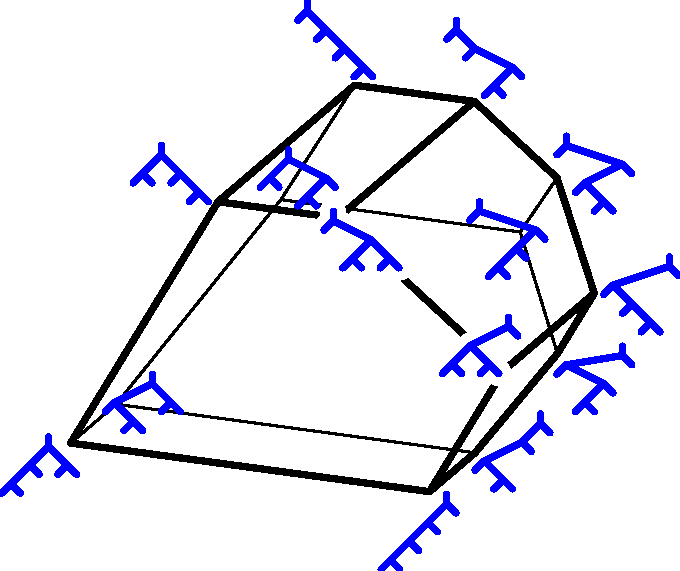
\includegraphics[scale=.78]{associahedronLoday}}
\vspace{-.4cm}
\papier{Loday ('04) \\ Hohlweg--Lange ('07) \\ Hohlweg--Lange--Thomas ('12) \\ Hohlweg--Pilaud--Stella ('18) \\ Pilaud--Santos--Ziegler ('24)

}
\end{minipage}
&&&
\begin{minipage}[t]{8.5cm}
\begin{center}
{\blue CHAP.--FOM.--ZEL.'S ASSOCIAHEDRON} \\[.5cm]
\end{center}
\centerline{\input{figures/associahedronCFZ}}
\vspace{-7.5cm}\hspace{5.3cm}
{\normalsize (Pictures by CFZ)}
\vspace{5.8cm}

\papier{Chapoton--Fomin--Zelevinsky ('02) \\ Ceballos--Santos--Ziegler ('11)

}
\end{minipage}
\end{tabular}

\end{slide}

%%%%%%%%%

\begin{slide}{THREE FAMILIES OF REALIZATIONS}

\vspace{-.25cm}
\hspace{-1.2cm}
\begin{tabular}{cc|ccc|cc}
\begin{minipage}[t]{8.5cm}
\begin{center}
{\blue SECONDARY} \\ {\blue POLYTOPE} \\[.5cm]
\end{center}
\vspace{-.2cm}
\centerline{\includegraphics[scale=1.5]{associahedron}}
\vspace{.1cm}
\papier{Gelfand--Kapranov--Zelevinsky ('94) \\ Billera--Filliman--Sturmfels ('90)

}
\vspace{.1cm}
\centerline{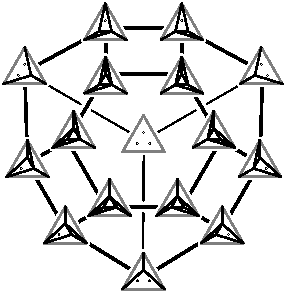
\includegraphics[scale=1.5]{secondaryPolytope}}
\vspace{1cm}
\end{minipage}
&&&
\begin{minipage}[t]{8.5cm}
\begin{center}
{\blue LODAY'S ASSOCIAHEDRON} \\[.5cm]
\end{center}
\vspace{-.2cm}
\centerline{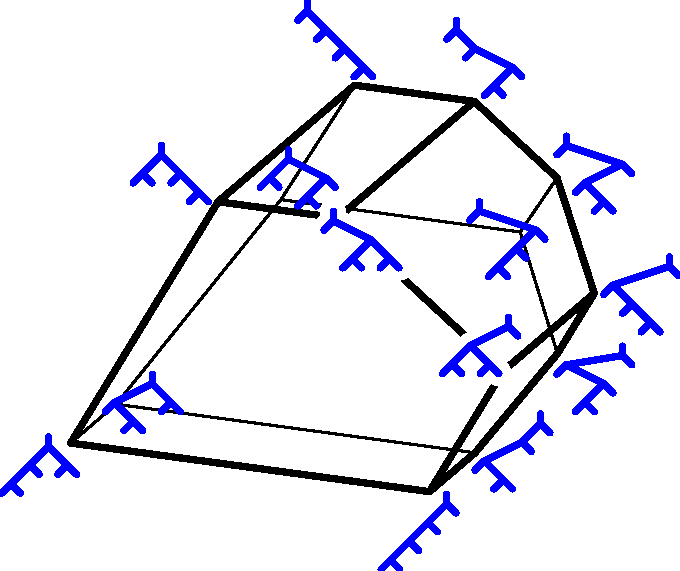
\includegraphics[scale=.78]{associahedronLoday}}
\vspace{-.4cm}
\papier{Loday ('04) \\ Hohlweg--Lange ('07) \\ Hohlweg--Lange--Thomas ('12) \\ Hohlweg--Pilaud--Stella ('18) \\ Pilaud--Santos--Ziegler ('24)

}
\vspace{.3cm}
\hspace{-.4cm}\boxed{\begin{minipage}{2.5cm} \smallskip \begin{center} \blue Hopf \\ algebra \\[-1.2cm] ~\end{center} \end{minipage}} \\[.2cm]
\hspace*{-.4cm}\boxed{\begin{minipage}{2.5cm} \smallskip \begin{center} \blue Cluster \\ algebras \\[-1.2cm] ~\end{center} \end{minipage}} \\
\vspace{-4.7cm}
\hspace*{3.5cm}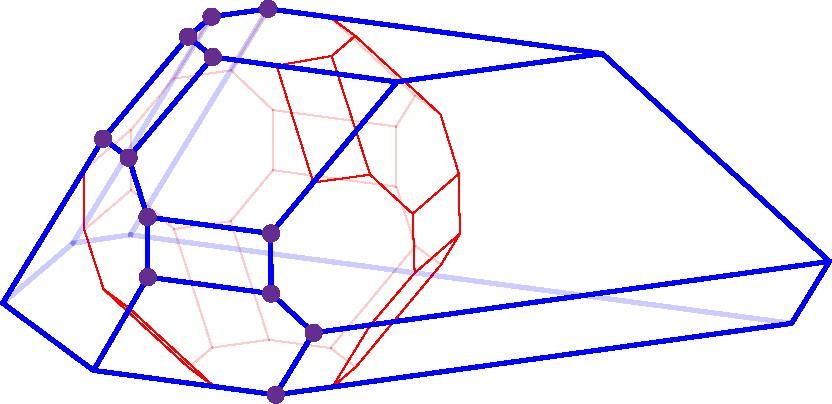
\includegraphics[scale=.35]{associahedronTypeB}
\vspace{-.2cm}
\hspace*{2.5cm}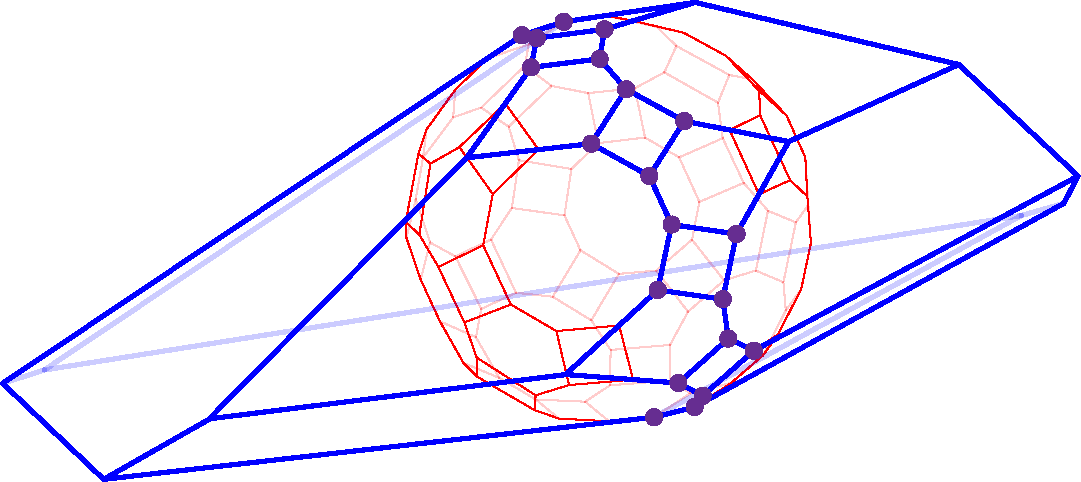
\includegraphics[scale=.35]{associahedronTypeH}
\end{minipage}
&&&
\begin{minipage}[t]{8.5cm}
\begin{center}
{\blue CHAP.--FOM.--ZEL.'S ASSOCIAHEDRON} \\[.5cm]
\end{center}
\centerline{\input{figures/associahedronCFZ}}
\vspace{-7.5cm}\hspace{5.3cm}
{\normalsize (Pictures by CFZ)}
\vspace{5.8cm}

\papier{Chapoton--Fomin--Zelevinsky ('02) \\ Ceballos--Santos--Ziegler ('11)

}
\vspace{1.2cm}
\hspace{-.4cm}\boxed{\begin{minipage}{2.5cm} \smallskip \begin{center} \blue Cluster \\ algebras \\[-1.2cm] ~\end{center} \end{minipage}} \\
\vspace{-3cm}
\centerline{\hspace{2.5cm}\setlength{\unitlength}{1.1pt} 
\begin{picture}(180,159)(0,0) 
\thicklines 

\put(0,0){\line(1,0){120}} 
\put(0,0){\line(0,1){50}} 
\put(120,0){\line(0,1){10}} 
\put(120,0){\line(1,1){60}} 
\put(0,50){\line(1,0){60}} 
\put(0,50){\line(1,2){50}} 
\put(120,10){\line(-1,1){20}} 
\put(120,10){\line(1,2){10}} 
\put(180,60){\line(0,1){20}} 
\put(60,50){\line(1,2){20}} 
\put(130,30){\line(1,1){50}} 
\put(130,30){\line(-1,1){20}} 
\put(100,30){\line(-2,1){40}} 
\put(100,30){\line(1,2){10}} 
\put(110,50){\line(-1,3){10}} 
\put(100,80){\line(-2,1){20}} 
\put(100,80){\line(0,1){40}} 
\put(80,90){\line(0,1){40}} 
\put(180,80){\line(-1,1){60}} 
\put(100,120){\line(-2,1){20}} 
\put(100,120){\line(1,1){20}} 
\put(80,130){\line(-1,2){10}} 
\put(50,150){\line(1,0){20}} 
\put(50,150){\line(1,1){10}} 
\put(70,150){\line(1,1){10}} 
\put(60,160){\line(1,0){20}} 
\put(80,160){\line(2,-1){40}} 
 
\thinlines 
\multiput(0,0)(3,3){20}{\circle*{0.5}} 
\multiput(60,60)(4,0){30}{\circle*{0.5}} 
\multiput(60,60)(0,4){25}{\circle*{0.5}} 
 
\put(65,155){\makebox(0,0){\blue \small $\alpha_2$}} 
\put(47,100){\makebox(0,0){\blue $\scriptstyle \alpha_1+\alpha_2$}} 
\put(135,85){\makebox(0,0){\blue $\scriptstyle \alpha_2+\alpha_3$}} 
\put(94,141){\makebox(0,0){\blue \small $2\alpha_2+\alpha_3$}} 
%\put(115,30){\makebox(0,0){$\scriptstyle \alpha_1+\alpha_2+\alpha_3$}} 
%\put(90,105){\makebox(0,0){$\begin{array}{c}\scriptstyle 
%\alpha_1+2\alpha_2\\ \scriptstyle+\alpha_3\end{array}$}} 
\put(57,25){\makebox(0,0){\blue $\scriptstyle \alpha_1$}} 
\put(150,40){\makebox(0,0){\blue $\scriptstyle \alpha_3$}} 
\put(87,65){\makebox(0,0){\blue \small $2\alpha_1+2\alpha_2+\alpha_3$}}  
\end{picture} 
}

\end{minipage}
\end{tabular}

\end{slide}

%%%%%%%%%
%
%\begin{slide}{LODAY'S ASSOCIAHEDRON}
%
%\vspace{-.3cm}
%\cboite{
%\vspace{-.7cm}
%\[
%\Asso(n) \, \eqdef \, \conv \set{\b{L}(T)}{T \text{ binary tree}} \, = \, \HH \; \cap \!\!\!\!\!\! \bigcap_{1 \le i \le j \le n+1} \!\!\!  \HS(i,j)
%\]
%\vspace{-.3cm}
%\[
%\b{L}(T) \eqdef \big[ \ell(T, i) \cdot r(T, i) \big]_{i \in [n+1]}
%\qquad
%\HS(i,j) \eqdef \biggset{\b{x} \in \R^{n+1}}{\sum_{i \le k \le j} x_i \ge \binom{j-i+2}{2} \!\! }
%\]
%
%\flushright{
%\papier{
%	Shnider-Sternberg, \textit{Quantum groups: From coalgebras to Drinfeld algebras} ('93) \\
%	Loday, \textit{Realization of the Stasheff polytope} ('04)
%	
%}}
%}
%
%\vspace{.3cm}
%\centerline{\raisebox{1cm}{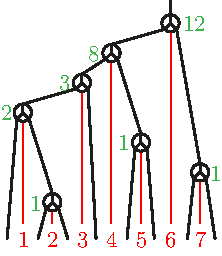
\includegraphics[scale=2.2]{LodayVector}} \qquad  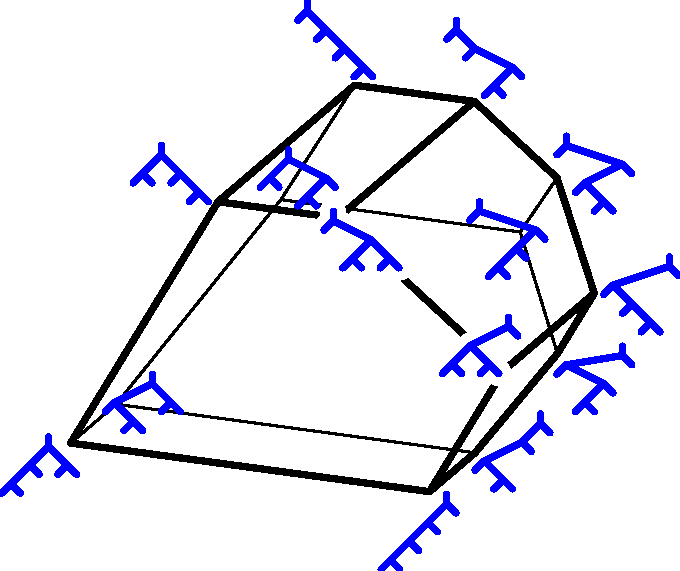
\includegraphics[scale=1.15]{associahedronLoday}}
%
%\end{slide}
%
%%%%%%%%%

\begin{slide}{LODAY'S ASSOCIAHEDRON}

\vspace*{-1cm}
\begin{align*}
\text{\blue Loday's associahedron} \; & = \; \conv \set{L(T)}{T \text{ triangulation of the } (n+3)\text{-gon}} \\
& = \; \HH \; \cap \!\!\!\!\! \bigcap_{\substack{\delta \text{ diagonal} \\ \text{of the } (n+3)\text{-gon}}} \!\!\!\!\!\!\!\!\!\! \HS(\delta)
\end{align*}

\vspace{-.5cm}
\centerline{
	\begin{overpic}[scale=2.5]{lodayTriangulation}
		\put(30,90){$i$}
		\put(175,0){$j$}
		\put(345,175){$k$}
		\put(53,23){$\ell(T,j)$}
		\put(295,55){$r(T,j)$}
		\put(560,140){$\delta$}
		\put(595,5){$B(\delta)$}
   \end{overpic}
}
\[
\hspace{1.8cm}
L(T) = \big(\ell(T,j) \, \cdot \, r(T,j)\big)_{j \in [n+1]}
\hspace{1.7cm}
\HS(\delta) = \biggset{\b{x} \in \R^{n+1}}{\sum_{j \in B(\delta)} x_j \ge \binom{|B(\delta)|+1}{2}}
\]

\vspace{.5cm}
\papier{Loday ('04)}

\end{slide}

%%%%%%%%%

\begin{slide}{HOHLWEG \& LANGE'S ASSOCIAHEDRA}

Can also replace Loday's $(n+3)$-gon by others\dots

\vspace{.2cm}
\centerline{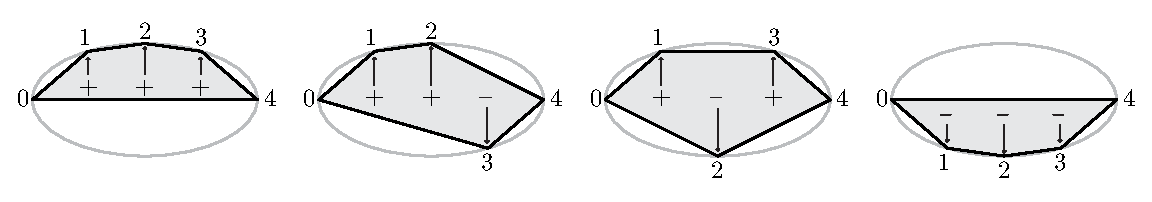
\includegraphics[width=\textwidth]{polygonsHohlwegLange}}

\vspace{-.3cm}
\dots to obtain different realizations of the associahedron

\vspace{.1cm}
\centerline{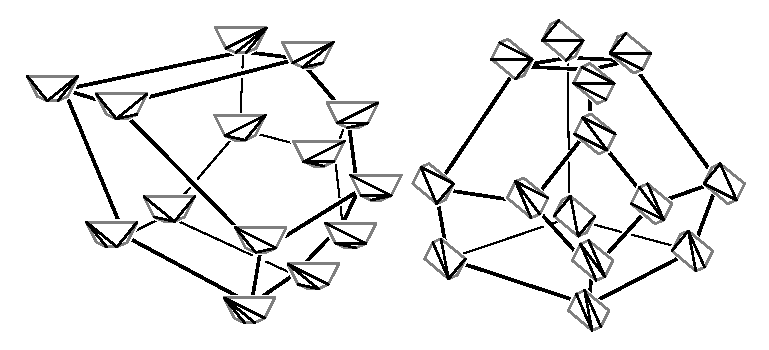
\includegraphics[scale=2]{associahedronLodayHL}}

\vspace{-.6cm}
\papier{Hohlweg--Lange ('07)}

\end{slide}

%%%%%%%%%

\begin{slide}{HOHLWEG \& LANGE'S ASSOCIAHEDRA}

\vspace*{-1cm}
\[
\Asso(P) \; = \; \conv \set{H\!L(T)}{T \text{ triangulation of } P} \; = \; \HH \; \cap \!\!\!\!\! \bigcap_{\delta \text{ diagonal of } P} \!\!\!\!\!\!\!\!\!\! \HS(\delta)
\]

\vspace{-.6cm}
\centerline{
	\begin{overpic}[scale=2.5]{hohlwegLange}
		\put(30,85){$i$}
		\put(85,325){$j$}
		\put(255,30){$k$}
		\put(-20,225){$\ell(T,j)$}
		\put(275,290){$r(T,j)$}
		\put(540,165){$\delta$}
		\put(370,110){$B(\delta)$}
   \end{overpic}
}

\vspace{-1.3cm}
\[
\hspace*{-1cm}
H\!L(T)_j =
\begin{cases}
	\ell(T,j) \cdot r(T,j) & \text{if } j \text{ down} \\
	n+2-\ell(T,j) \cdot r(T,j) & \text{if } j \text{ up}
\end{cases}
\hspace{1.4cm}
\HS(\delta) = \biggset{\b{x}}{\sum_{j \in B(\delta)} x_j \ge \binom{|B(\delta)|+1}{2}}
\]

\papier{Hohlweg--Lange ('07)}

\end{slide}

%%%%%%%%%%%%%%%%%%%%%%%%%%%%%%%%%%%%%%%%%%%%%%%%%%%%%%

\partie{Pseudotriangulations \& PPT polytope}

\begin{slide}{Three geometric structures}

\hspace{1.6cm} triangulations \hspace{3.4cm} pseudotriangulations \hspace{2.5cm} multitriangulations\\
\begin{center}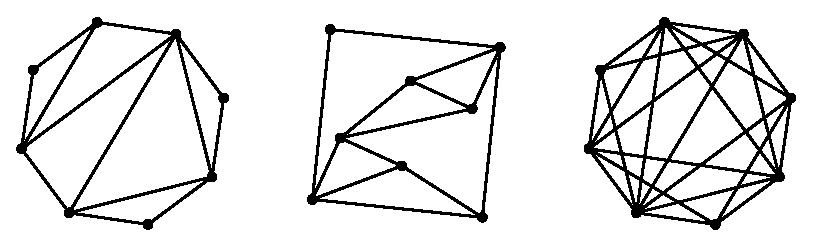
\includegraphics[scale=1.9]{geometricStructures0}\end{center}
\vspace{-1.08cm} \hspace*{25.7cm} ${k=2}$

\hspace{1.7cm} 
\begin{tabular}[t]{c} crossing-free \\ \\[-.3cm] \\ \\  \end{tabular} 
\hspace{3.4cm} 
\begin{tabular}[t]{c} crossing-free pointed \\ \papier{Pocchiola--Vegter ('96)} \\[-.3cm] \papier{Rote--Santos--Streinu ('08)} \\ \\  \end{tabular}
\hspace{2cm} 
\begin{tabular}[t]{c} $(k+1)$-crossing-free \\ \papier{Capoyleas--Pach ('92)} \\[-.3cm] \papier{Jonsson ('05)} \\ \\ \\  \end{tabular}

\end{slide}

%%%

\begin{slide}{Three geometric structures}

\hspace{1.6cm} triangulations \hspace{3.4cm} pseudotriangulations \hspace{2.5cm} multitriangulations\\
\begin{center}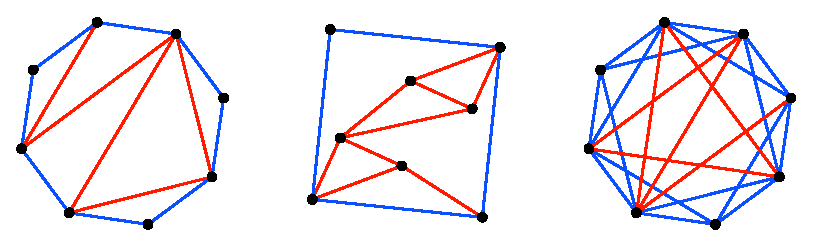
\includegraphics[scale=1.9]{geometricStructures1}\end{center}
\vspace{-1.08cm} \hspace*{25.7cm} ${k=2}$

\hspace{1.7cm} 
\begin{tabular}[t]{c} crossing-free \\ \\[-.3cm] \\ \\  \end{tabular} 
\hspace{3.4cm} 
\begin{tabular}[t]{c} crossing-free pointed \\ \papier{Pocchiola--Vegter ('96)} \\[-.3cm] \papier{Rote--Santos--Streinu ('08)} \\ \\  \end{tabular}
\hspace{2cm} 
\begin{tabular}[t]{c} $(k+1)$-crossing-free \\ \papier{Capoyleas--Pach ('92)} \\[-.3cm] \papier{Jonsson ('05)} \\ \\ \\  \end{tabular}

\end{slide}

%%%

\begin{slide}{Three geometric structures}

\hspace{1.6cm} triangulations \hspace{3.4cm} pseudotriangulations \hspace{2.5cm} multitriangulations\\
\begin{center}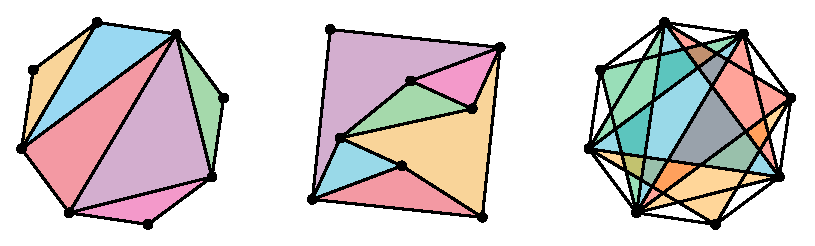
\includegraphics[scale=1.9]{geometricStructures2}\end{center}
\vspace{-1.08cm} \hspace*{25.7cm} ${k=2}$

\hspace{1.7cm} 
\begin{tabular}[t]{c} crossing-free \\ \\[-.3cm] \\ \\ triangles \end{tabular} 
\hspace{3.4cm} 
\begin{tabular}[t]{c} crossing-free pointed \\ \papier{Pocchiola--Vegter ('96)} \\[-.3cm] \papier{Rote--Santos--Streinu ('08)} \\ \\ pseudotriangles \end{tabular}
\hspace{2cm} 
\begin{tabular}[t]{c} $(k+1)$-crossing-free \\ \papier{Capoyleas--Pach ('92)} \\[-.3cm] \papier{Jonsson ('05)} \\ \\ $k$-stars \\ \papier{P.--Santos ('09)} \end{tabular}

\end{slide}

%%%

\begin{slide}{Three geometric structures}

\hspace{1.6cm} triangulations \hspace{3.4cm} pseudotriangulations \hspace{2.5cm} multitriangulations\\
\begin{center}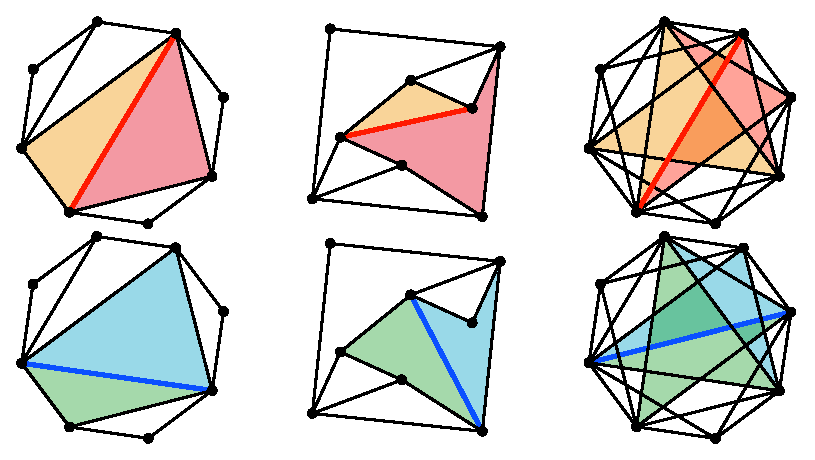
\includegraphics[scale=1.9]{geometricStructures3}\end{center}
\vspace{-8cm} \hspace*{25.7cm} ${k=2}$

\vspace{7cm}
\begin{center}
\emph{flip} = exchange an internal edge with the common bisector of the two adjacent cells
\end{center}

\end{slide}

%%%

\begin{slide}{Three geometric structures}

\hspace{1.6cm} triangulations \hspace{3.4cm} pseudotriangulations \hspace{2.5cm} multitriangulations
\begin{center}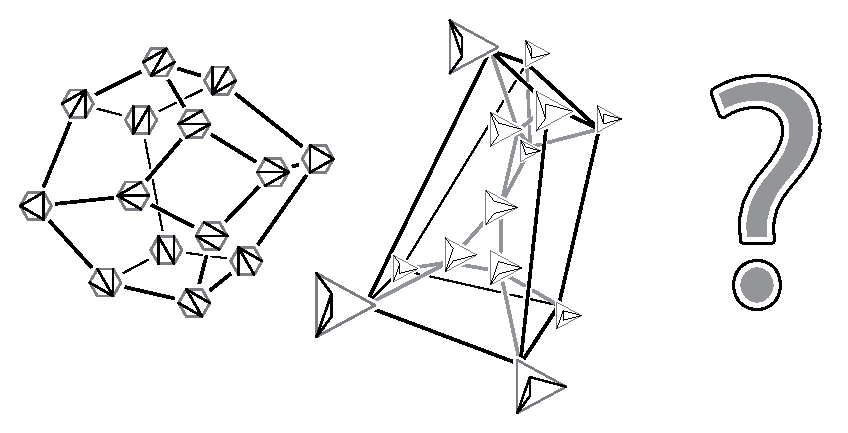
\includegraphics[width=.95\textwidth]{geometricStructures4}\hspace*{1.5cm}~\end{center}
\hspace{1.5cm} associahedron \hspace{2.4cm} \begin{tabular}[t]{c}pseudotriangulation polytope \\  \papier{Rote--Santos--Streinu ('03)} \end{tabular} \hspace{1cm} multiassociahedron

\vspace{-1cm}
\end{slide}

%\begin{slide}{Three geometric structures}
%\vspace{-.8cm}
%\hspace{1.6cm} triangulations \hspace{3.4cm} pseudotriangulations \hspace{2.5cm} multitriangulations
%\begin{center}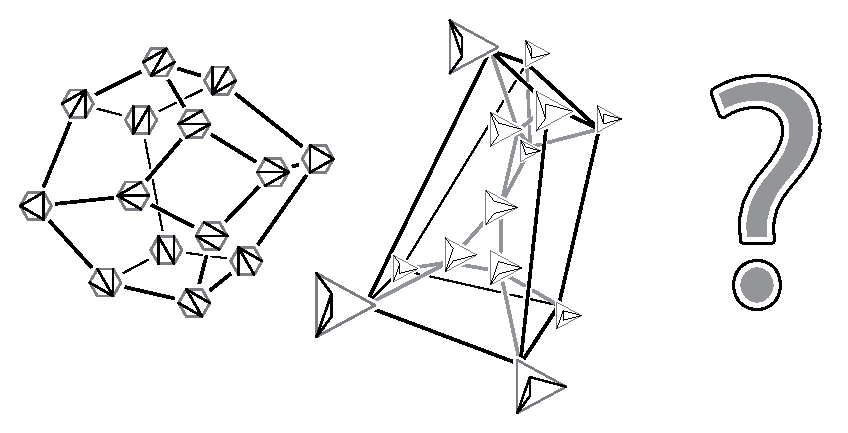
\includegraphics[width=.95\textwidth]{geometricStructures4}\hspace*{1.5cm}~\end{center}
%
%\vspace{-.7cm}
%\begin{flushright}
%``Our main limits in understanding the combinatorial structure of polytopes still\\
%lie in our ability to raise the good questions and in the \emph{lack of examples},\\
%\emph{methods of constructing them}, and \emph{means of classifying them}.'' \\
%\papier{G. Kalai, \emph{Handbook of Discrete \& Computational Geometry}.}
%\end{flushright}
%
%\vspace{-2cm}
%\end{slide}

%%%%%%%

%\begin{slide}{LINE SPACE OF THE PLANE = M\"OBIUS STRIP}
%
%\centerline{\includegraphics[angle=-90,scale=2]{MoebiusBand}}
%
%\end{slide}
%
%%%%%%%%
%
%\multido{\n=0+1}{10}{%
%\begin{slide}{Duality}
%\hspace{1.6cm} triangulations \hspace{3.4cm} pseudotriangulations \hspace{2.5cm} multitriangulations\\
%\vspace{-.5cm}\\
%\vspace*{-2cm}
%\hspace*{-.6cm}\includegraphics[scale=1.9]{geometricStructures5\n}\\
%\vspace{-8.5cm} \\ \hspace*{25.7cm} ${k=2}$
%\end{slide}
%}
%
%%%%

\begin{slide}{Duality}
\hspace{1.6cm} triangulations \hspace{3.4cm} pseudotriangulations \hspace{2.5cm} multitriangulations\\
\vspace{-.5cm}\\
\vspace*{-2cm}
\hspace*{-.6cm}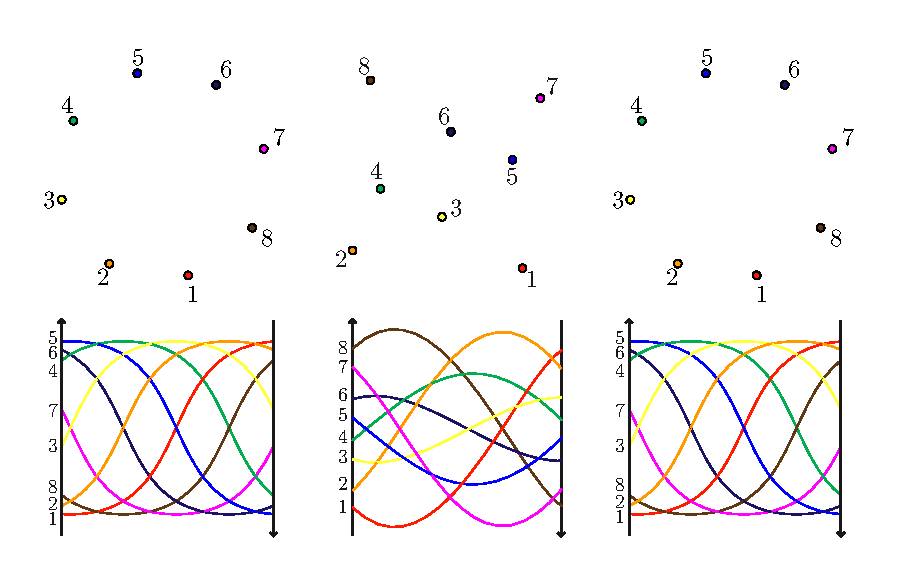
\includegraphics[scale=1.9]{geometricStructures5}
\vspace{-8.5cm} \\ \hspace*{25.7cm} ${k=2}$

\vspace{7.6cm}
\papier{P.--Pocchiola ('12)}

\vspace*{-3cm}
\end{slide}

%%%

\begin{slide}{Duality}
\hspace{1.6cm} triangulations \hspace{3.4cm} pseudotriangulations \hspace{2.5cm} multitriangulations\\
\vspace{-.5cm}\\
\vspace*{-2cm}
\hspace*{-.6cm}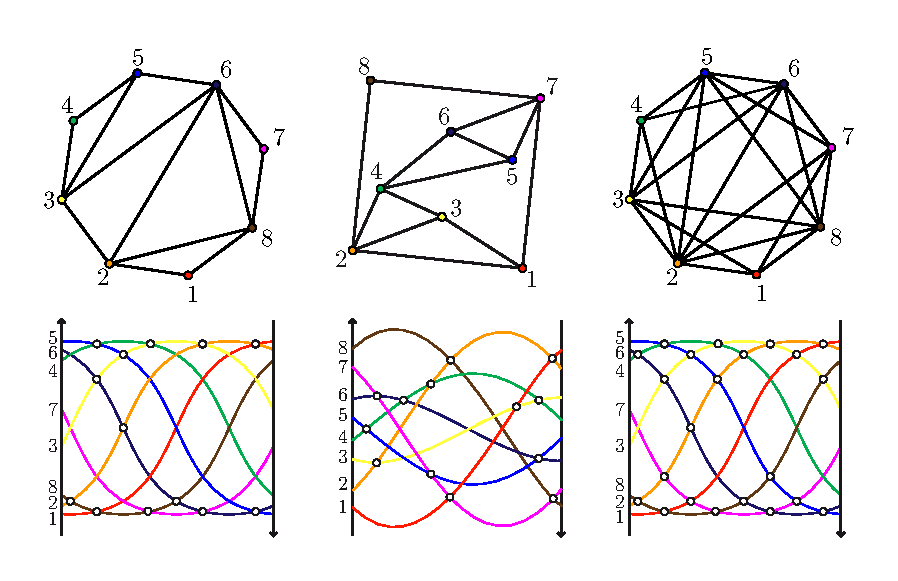
\includegraphics[scale=1.9]{geometricStructures6}
\vspace{-8.5cm} \\ \hspace*{25.7cm} ${k=2}$

\vspace{7.6cm}
\papier{P.--Pocchiola ('12)}

\vspace*{-3cm}
\end{slide}

%%%%
%
%\multido{\n=0+1}{10}{%
%\begin{slide}{Duality}
%\hspace{1.6cm} triangulations \hspace{3.4cm} pseudotriangulations \hspace{2.5cm} multitriangulations\\
%\vspace{-.5cm}\\
%\vspace*{-2cm}
%\hspace*{-.6cm}\includegraphics[scale=1.9]{geometricStructures7\n}
%\vspace{-8.5cm} \\ \hspace*{25.7cm} ${k=2}$
%\end{slide}
%}
%
%%%%

\begin{slide}{Duality}
\hspace{1.6cm} triangulations \hspace{3.4cm} pseudotriangulations \hspace{2.5cm} multitriangulations\\
\vspace{-.5cm}\\
\vspace*{-2cm}
\hspace*{-.6cm}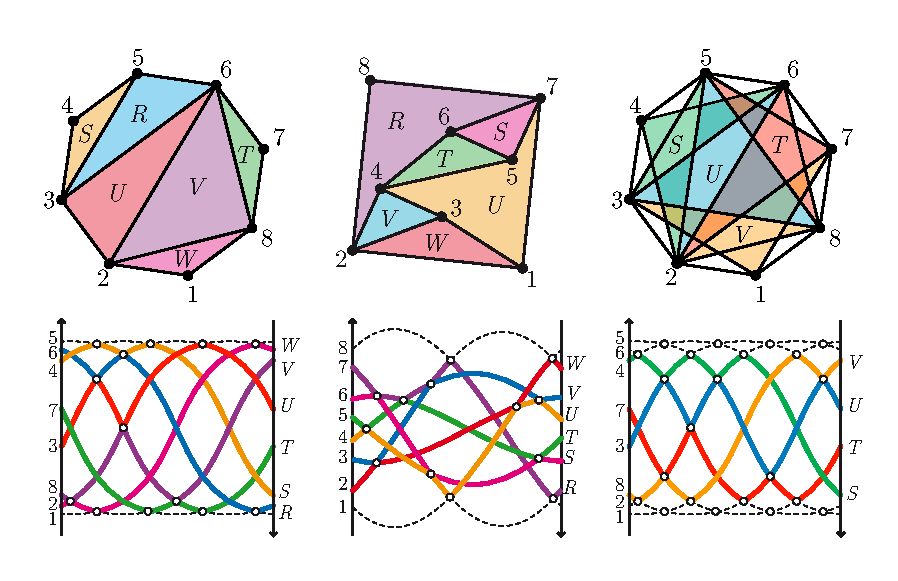
\includegraphics[scale=1.9]{geometricStructures7}
\vspace{-8.5cm} \\ \hspace*{25.7cm} ${k=2}$

\vspace{7.6cm}
\papier{P.--Pocchiola ('12)}

\vspace*{-3cm}
\end{slide}

%%%%%%%%%%
%
%\begin{slide}{Duality}
%\hspace{1.6cm} triangulations \hspace{3.4cm} pseudotriangulations \hspace{2.5cm} multitriangulations
%
%\vspace{1.3cm}
%\begin{center}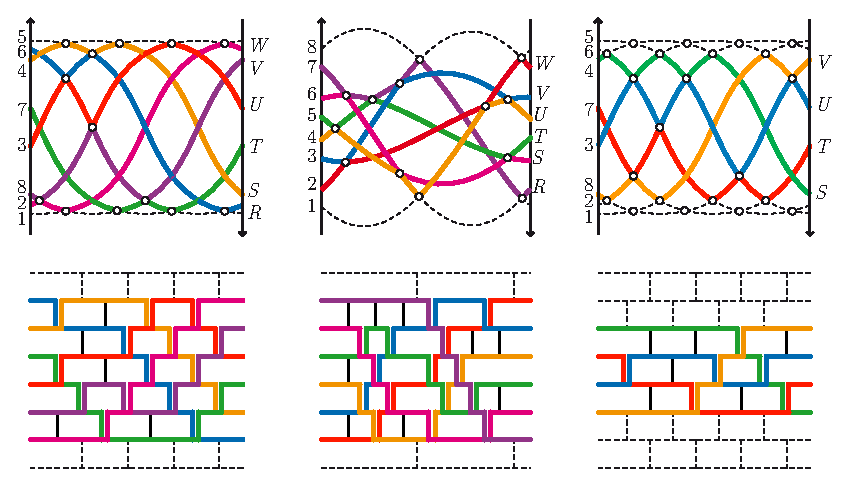
\includegraphics[scale=1.9]{geometricStructures8}\end{center}
%\vspace{-8.33cm} \hspace*{25.7cm} ${k=2}$
%\end{slide}

%%%%%%%%%%%%%%%%%%%%%%%%%%%%%%%%%%%%%%%%%%%%%%%%%%%%%%

\partie{Wiggly pseudotriangulations \& wiggly complex}

%%%%%%%%%%%%%%%%%%%%%%%%%%%%%%%%%%%%%%%%%%%%%%%%%%%%%%

\begin{slide}{Wiggly complex}

\emph{wiggly dissection} $=$ set of pairwise \emph{non-crossing} and \emph{pointed} wiggly arcs on $n+2$ points

\hspace{9.3cm}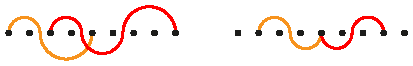
\includegraphics[scale=1.7]{incompatible}

\vspace{.2cm}
\emph{wiggly complex}~$\wigglyComplex_n$ $=$ simplicial complex of wiggly dissections

\vspace{.2cm}
\centerline{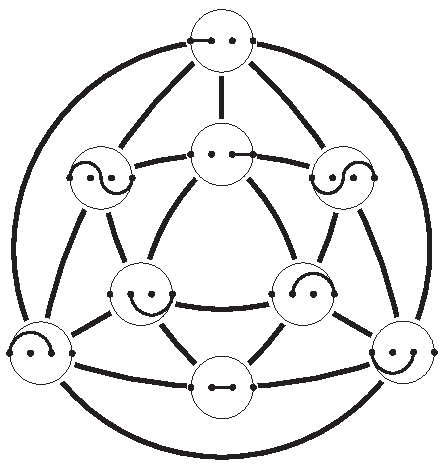
\includegraphics[scale=1.7]{wigglyComplex}}

%\theo{PROP}{The wiggly complex is a pure $(2n-1)$-dimensional pseudomanifold.}

\end{slide}

%%%

\begin{slide}{Wiggly complex}

\emph{wiggly dissection} $=$ set of pairwise \emph{non-crossing} and \emph{pointed} wiggly arcs on $n+2$ points

\hspace{9.3cm}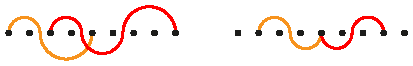
\includegraphics[scale=1.7]{incompatible}

\vspace{.2cm}
\emph{wiggly complex}~$\wigglyComplex_n$ $=$ simplicial complex of wiggly dissections

\begin{align*}
f(\wigglyComplex_1) & = (1, 2) \\
f(\wigglyComplex_2) & = (1, 9, 21, 14) \\
f(\wigglyComplex_3) & = (1, 24, 154, 396, 440, 176) \\
f(\wigglyComplex_4) & = (1, 55, 729, 4002, 10930, 15684, 11312, 3232) \\
f(\wigglyComplex_5) & = (1, 118, 2868, 28110, 140782, 400374, 673274, 662668, 352728, 78384) \\[.8cm]
h(\wigglyComplex_1) & = (1, 1) \\
h(\wigglyComplex_2) & = (1, 6, 6, 1) \\
h(\wigglyComplex_3) & = (1, 19, 68, 68, 19, 1) \\
h(\wigglyComplex_4) & = (1, 48, 420, 1147, 1147, 420, 48, 1) \\
h(\wigglyComplex_5) & = (1, 109, 1960, 11254, 25868, 25868, 11254, 1960, 109, 1)
\end{align*}

\end{slide}

%%%%%%%%%%%%%%%%%%%%%%%%%%%%%%%%%%%%%%%%%%%%%%%%%%%%%%

\begin{slide}{Wiggly pseudotriangulations}

$c$ cell in a wiggly dissection with boundary $\partial_c$ \\
\emph{degree} $\delta_c =  1/2 \, \# \text{arcs on } \partial_c + 2 \, \# \text{connected components of } \partial_c - 1$ \\
\emph{pseudotriangle} $=$ cell of degree $3$ \qquad \emph{pseudoquadrangle} $=$ cell of degree $4$

\vspace{.4cm}
\centerline{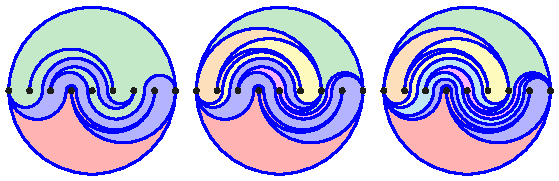
\includegraphics[scale=3]{wigglyPseudodissections}}

\vspace{.1cm}
\theo{PROP}{The inclusion maximal wiggly pseudodissections are the pseudotriangulations, and contain $2n-1$ internal arcs and $n$ cells. \hfill \papier{Bapat--P. (24$^+$)}

}

\vspace{.3cm}
%$wp_n = \#$wiggly pseudotriangulations
\[
\begin{array}{c|ccccccccc}
n & 1 & 2 & 3 & 4 & 5 & 6 & 7 & 8 & \dots \\
\hline
wp_n & 2 & 14 & 176 & 3232 & 78384 & 2366248 & 85534176 & 3602770400 & \dots
\end{array}
\]

\end{slide}

%%%%%%%%%%%%%%%%%%%%%%%%%%%%%%%%%%%%%%%%%%%%%%%%%%%%%%

\begin{slide}{Wiggly flip graph}

\theo{PROP}{Any wiggly pseudoquadrangle has exactly two wiggly diagonals, and they either cross or are non pointed. \hfill \papier{Bapat--P. (24$^+$)}

}

\vspace{.1cm}
\centerline{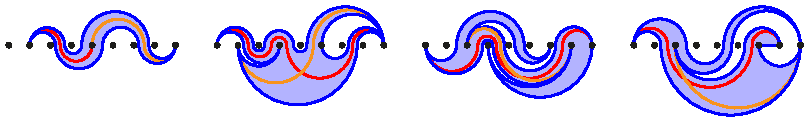
\includegraphics[scale=2]{diagonalsPseudoquadrangles}}

\end{slide}

%%%

\begin{slide}{Wiggly flip graph}

\theo{PROP}{Any wiggly pseudoquadrangle has exactly two wiggly diagonals, and they either cross or are non pointed. \hfill \papier{Bapat--P. (24$^+$)}

}

\vspace{.1cm}
\centerline{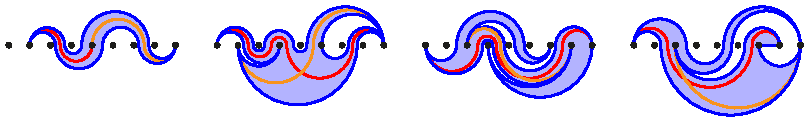
\includegraphics[scale=2]{diagonalsPseudoquadrangles}}

\vspace{-.4cm}
\emph{wiggly flip graph} $\wigglyFlipGraph_n =$ \begin{tabular}[t]{|ll} a vertex for each wiggly pseudotriangulation \\ an edge between~$T$ and~$T'$ if~$T \ssm \{\alpha\} = T' \ssm \{\alpha'\}$ \end{tabular}

\vspace{.3cm}
\centerline{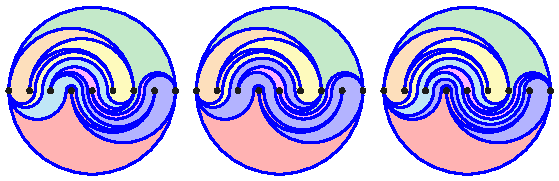
\includegraphics[scale=3]{wigglyFlip}}

\end{slide}

%%%

\begin{slide}{Wiggly flip graph}

\vspace{.5cm}
\theo{PROP}{The wiggly flip graph $\wigglyFlipGraph_n$ is $(2n-1)$-regular and connected. \hfill \papier{Bapat--P. (24$^+$)}

}

\vspace{.5cm}
\centerline{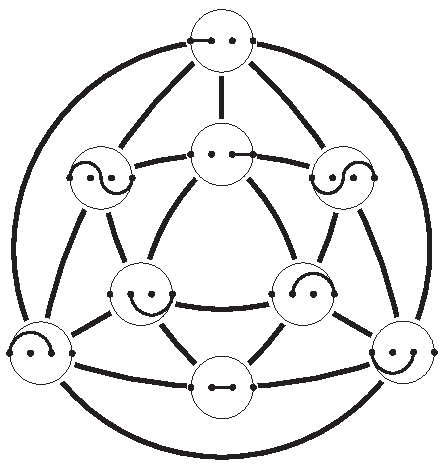
\includegraphics[scale=1.7]{wigglyComplex} \hspace{-2cm} 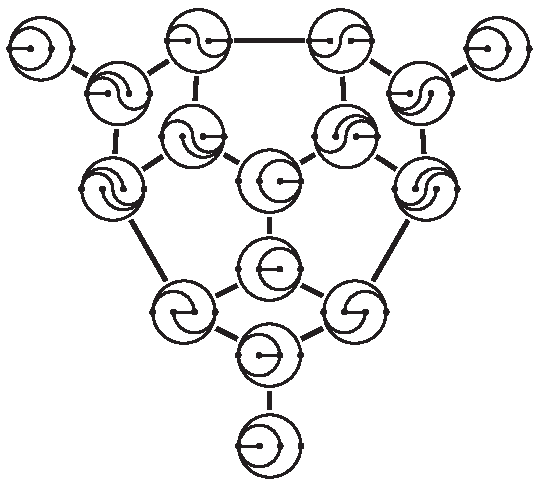
\includegraphics[scale=1.7]{wigglyComplexDual}}

\end{slide}

%%%%%%%%%%%%%%%%%%%%%%%%%%%%%%%%%%%%%%%%%%%%%%%%%%%%%%

\partie{Wiggly permutations \& wiggly lattice}

%%%%%%%%%%%%%%%%%%%%%%%%%%%%%%%%%%%%%%%%%%%%%%%%%%%%%%

\begin{slide}{Wiggly permutations}

\vspace{1cm}
\hspace{13.5cm}
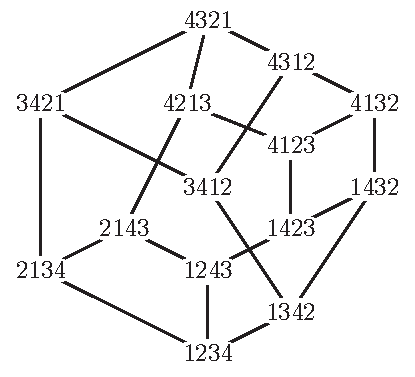
\includegraphics[scale=2]{wigglyLattice}

\vspace{-13.5cm}
\emph{wiggly permutation} = permutation of $2n$ avoiding
\begin{compactitem}
\item $(2j-1) \cdots i \cdots (2j)$ for~$j \in [n]$ and~$i < 2j-1$,
\item $(2j) \cdots k \cdots (2j-1)$ for~$j \in [n]$ and~$k > 2j$.
\end{compactitem}

\vspace{1cm}
\begin{minipage}{13.2cm}
\theo{PROP}{
The wiggly permutations induce a sublattice~$\wigglyLattice_n$ of the weak order on~$\f{S}_{2n}$.

\hfill \papier{Bapat--P. (24$^+$)}

}

\theo{PROP}{
The cover graph of the lattice~$\wigglyLattice_n$ is $(2n-1)$-regular and connected.

\hfill \papier{Bapat--P. (24$^+$)}

}
\end{minipage}

\vspace{3cm}
\[
\begin{array}{c|ccccccccc}
n & 1 & 2 & 3 & 4 & 5 & 6 & 7 & 8 & \dots \\
\hline
wp_n & 2 & 14 & 176 & 3232 & 78384 & 2366248 & 85534176 & 3602770400 & \dots
\end{array}
\]

\end{slide}

%%%%%%%%%%%%%%%%%%%%%%%%%%%%%%%%%%%%%%%%%%%%%%%%%%%%%%

\begin{slide}{Wiggly pseudotriangulations $\longleftrightarrow$ wiggly permutations}

\vspace{1cm}
\centerline{
\includegraphics[scale=1.42]{wigglyPseudotriangulations}}
\vspace{-.3cm}
\centerline{$
1234 \;\;\; 1243 \;\;\; 1342 \;\;\; 1423 \;\;\; 1432 \;\;\; 2134 \;\;\; 2143 \;\;\; 3412 \;\;\; 3421 \;\;\; 4123 \;\;\; 4132 \;\;\; 4213 \;\;\; 4312 \;\;\; 4321
$}

\vspace{1cm}
\theo{PROP}{The wiggly pseudotriangulations and wiggly permutations are in bijection.

\hfill \papier{Bapat--P. (24$^+$)}

}

\vspace{.5cm}
\centerline{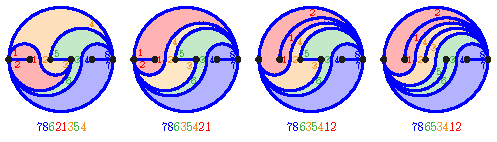
\includegraphics[scale=3.3]{bijection}}

{\color{gray}
permutation of $2n$ avoiding \begin{tabular}[t]{@{}l} $(2j-1) \cdots i \cdots (2j)$ for~$j \in [n]$ and~$i < 2j-1$ \\ $(2j) \cdots k \cdots (2j-1)$ for~$j \in [n]$ and~$k > 2j$ \end{tabular}}

\end{slide}

%%%

\begin{slide}{Wiggly pseudotriangulations $\longleftrightarrow$ wiggly permutations}

\theo{PROP}{This bijection induces a directed graph isomorphism between
\begin{compactitem}
\item the wiggly increasing flip graph on wiggly pseudotriangulations,
\item the Hasse diagram of the wiggly lattice on wiggly permutations. \hfill \papier{Bapat--P. (24$^+$)}
\end{compactitem}
}

\vspace{.5cm}
\centerline{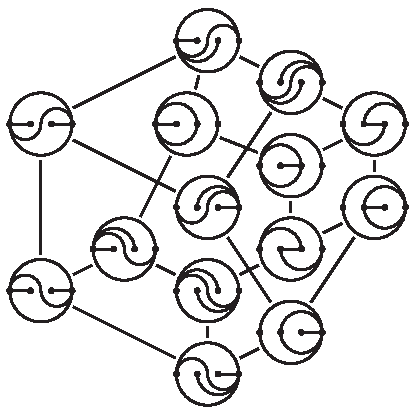
\includegraphics[scale=1.8]{wigglyFlipGraph}\quad\raisebox{.5cm}{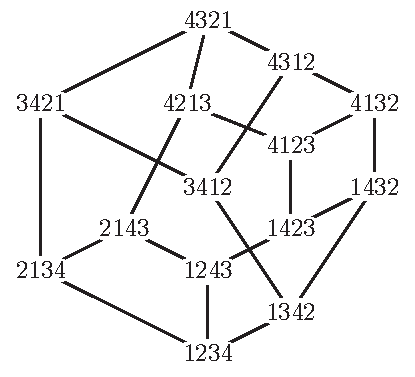
\includegraphics[scale=1.8]{wigglyLattice}}}

\end{slide}

%%%%%%%%%%%%%%%%%%%%%%%%%%%%%%%%%%%%%%%%%%%%%%%%%%%%%%

\partie{Wiggly fan}

%%%%%%%%%%%%%%%%%%%%%%%%%%%%%%%%%%%%%%%%%%%%%%%%%%%%%%

\begin{slide}{g- and c-vectors}

\emph{$\b{g}$-vector} of $\alpha =$ proj. on $\sum_{i = 1}^{2n} x_i = 0$ of \raisebox{-1.7cm}{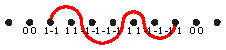
\includegraphics[scale=4]{gvector}}

\vspace{-.5cm}
\emph{$\b{c}$-vector} of~$\alpha \in T = $ you don't want to know...

\vspace{.5cm}
\theo{PROP}{For any wiggly pseudotriangulation~$T$, the $\b{g}$-vectors~$\set{\b{g}(\alpha)}{\alpha \in T^\circ}$ and the $\b{c}$-vectors~$\set{\b{c}(\alpha, T)}{\alpha \in T^\circ}$ form dual bases. \hfill \papier{Bapat--P. (24$^+$)}

}

\vspace{1cm}
\centerline{\raisebox{-4cm}{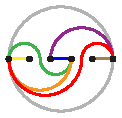
\includegraphics[scale=4]{pseudotriangulationMatrices}} \quad \(
\begin{blockarray}{ccccccccc}
	& & {\color{brown} \bullet} & {\color{red} \bullet} & {\color{orange} \bullet} & {\color{yellow} \bullet} & {\color{green} \bullet} & {\color{blue} \bullet} & {\color{violet} \bullet} \\
	\begin{block}{c@{\hspace*{-.1cm}}c(ccccccc)}
	1 & & 0 & \! -1/2 \!\! & \!\! -1/2 \!\! & -1 & 1 & 0 & \!\! -1/2 \\
	2 & & 0 & \! -1/2 \!\! & \!\! -1/2 \!\! & 1 & 1 & 0 & \!\! -1/2 \\
	3 & & 0 & \! -1/2 \!\! & \!\! -1/2 \!\! & 0 & \; -1 \; & 1 & 1/2 \\
	4 & & 0 & \! -1/2 \!\! & \!\! -1/2 \!\! & 0 & \; -1 \; & -1\!\! & \!\!\! -3/2 \\
	5 & & 0 & \! -1/2 \!\! & \!\! -1/2 \!\! & 0 & \; -1 \; & -1 \!\! & 1/2 \\
	6 & & 0 & \! -1/2 \!\! & 3/2 & 0 & 1 & 1 & 1/2 \\
	7 & & 1 & 3/2 & 1/2 & 0 & 0 & 0 & 1/2 \\
	8 & & -1 \!\! & 3/2 & 1/2 & 0 & 0 & 0 & 1/2 \\
	\end{block}
	& & & & \multicolumn{2}{c}{$\b{g}(T)$} & &
\end{blockarray}
%
\qquad
%
\begin{blockarray}{ccccccccc}
	& & {\color{brown} \bullet} & {\color{red} \bullet} & {\color{orange} \bullet} & {\color{yellow} \bullet} & {\color{green} \bullet} & {\color{blue} \bullet} & {\color{violet} \bullet} \\
	\begin{block}{c@{\hspace*{-.1cm}}c(ccccccc)}
	1 & & 0 & 0 & \!\! -1/4 \!\! & 1/2 & 1/4 & 0 & 0 \\
	2 & & 0 & 0 & \!\! -1/4 \!\! & \!\! -1/2 \!\! & 1/4 & 0 & 0 \\
	3 & & 0 & 0 & \!\! -1/4 \!\! & 0 & \!\! -1/4 \!\! & 1/2 & 0 \\
	4 & & 0 & 0 & 1/4 & 0 & \!\! -1/4 \!\! & 0 & \!\! -1/2 \! \\
	5 & & 0 & \!\! -1/4 \!\! & 0 & 0 & 0 & \!\! -1/2 \!\! & 1/2 \\
	6 & & 0 & \!\! -1/4 \!\! & 1/2 & 0 & 0 & 0 & 0 \\
	7 & & 1/2 & 1/4 & 0 & 0 & 0 & 0 & 0 \\
	8 & & -1/2 \!\!\! & 1/4 & 0 & 0 & 0 & 0 & 0 \\
	\end{block}
	& & & & \multicolumn{2}{c}{$\b{c}(T)$} & &
\end{blockarray}
\)}

\end{slide}

%%%%%%%%%%%%%%%%%%%%%%%%%%%%%%%%%%%%%%%%%%%%%%%%%%%%%%

\begin{slide}{wiggly fan}

\emph{$\b{g}$-vector} of $\alpha =$ proj. on $\sum_{i = 1}^{2n} x_i = 0$ of \raisebox{-1.7cm}{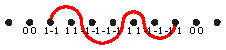
\includegraphics[scale=4]{gvector}}

\vspace{.1cm}
\theo{THM}{The cones~$\setangle{\b{g}(\alpha)}{\alpha \in D}$ for all wiggly dissections~$D$ form a complete simplicial fan~$\wigglyFan_n$ (in $\sum_{i = 1}^{2n} x_i = 0$). \hfill \papier{Bapat--P. (24$^+$)}

}

\vspace{2cm}
Main observation:

\centerline{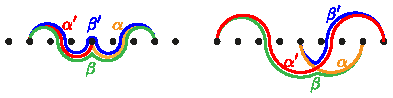
\includegraphics[scale=3.2]{incompatible2}}
\centerline{
${\red \b{g}(\alpha)} + {\orange \b{g}(\alpha')} = \big( {\green \b{g}(\beta)} + {\blue \b{g}(\beta')} \big) / 2$
\qquad
${\red \b{g}(\alpha)} + {\orange \b{g}(\alpha')} = {\green \b{g}(\beta)} + {\blue \b{g}(\beta')}$
}

\end{slide}

%%%%%%%%%%%%%%%%%%%%%%%%%%%%%%%%%%%%%%%%%%%%%%%%%%%%%%

\partie{Wigglyhedron}

%%%%%%%%%%%%%%%%%%%%%%%%%%%%%%%%%%%%%%%%%%%%%%%%%%%%%%

\begin{slide}{Wigglyhedron}

\emph{incompatibility degree}~$\delta(\alpha, \alpha') =$ 
\begin{compactitem}
\item $0$ if~$\alpha$ and~$\alpha'$ are pointed and non-crossing,
\item $1$ is~$\alpha$ and~$\alpha'$ are not pointed,
\item the number of crossings of~$\alpha$ and~$\alpha'$ if they are crossing.
\end{compactitem}

\vspace{.5cm}
$\kappa(\alpha) =$ \emph{incompatibility number} of~$\alpha = \sum_{\alpha'} \delta(\alpha, \alpha')$.

\vspace{2cm}
Main observation:

\centerline{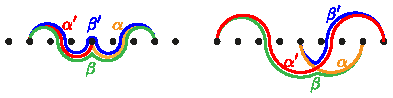
\includegraphics[scale=3.2]{incompatible2}}
\centerline{
${\red \kappa(\alpha)} + {\orange \kappa(\alpha')} > \big( {\green \kappa(\beta)} + {\blue \kappa(\beta')} \big) / 2$
\qquad
${\red \kappa(\alpha)} + {\orange \kappa(\alpha')} > {\green \kappa(\beta)} + {\blue \kappa(\beta')}$
}

\vspace{1.5cm}
Hence, $\kappa$ satisfies all wall-crossing inequalities of the wiggly fan...

\end{slide}

%%%%%%%%%%%%%%%%%%%%%%%%%%%%%%%%%%%%%%%%%%%%%%%%%%%%%%

\begin{slide}{Wigglyhedron}

\theo{THM}{
The wiggly fan~$\wigglyFan_n$ is the normal fan of a simplicial $(2n-1)$-dimensional polytope, called the \emph{wigglyhedron}~$\wigglyhedron_n$, and defined equivalently~as
\begin{itemize}
\item intersection of the halfspaces~$\set{\b{x} \in \R^{2n}}{\dotprod{\b{g}(\alpha)}{\b{x}} \!\le\! \kappa(\alpha)}$ for all wiggly arcs~$\alpha$,
\item convex hull of~$\b{p}(T) \eqdef \sum\limits_{\alpha \in T} \kappa(\alpha) \, \b{c}(\alpha, T)$ for all wiggly pseudotriangulations~$T$.
\end{itemize}

\vspace{-.6cm}
\hfill \papier{Bapat--P. (24$^+$)}

}

\vspace{.5cm}
\centerline{\begin{tikzpicture}%
	[x={(0.681462cm, -0.327528cm)},
	y={(0.731633cm, 0.326817cm)},
	z={(-0.017949cm, 0.886519cm)},
	scale=.900000,
	back/.style={color=blue, thin},
	edge/.style={color=blue, very thick, },
	facet/.style={fill=blue,fill opacity=0.00000},
	vertex/.style={inner sep=1pt,circle,draw=blue,fill=blue,thick}]
%
%
%% This TikZ-picture was produce with Sagemath version 9.5
%% with the command: ._tikz_3d_in_3d and parameters:
%% view = [-764, -346, -545]
%% angle = 76.39
%% scale = 1
%% edge_color = blue
%% facet_color = blue
%% opacity = 0.5
%% vertex_color = blue
%% axis = False

%% Coordinate of the vertices:
%%
\coordinate (-1.00000, -4.00000, -3.00000) at (-1.00000, -4.00000, -3.00000);
\coordinate (1.00000, 0.00000, -3.00000) at (1.00000, 0.00000, -3.00000);
\coordinate (3.00000, 4.00000, 1.00000) at (3.00000, 4.00000, 1.00000);
\coordinate (3.00000, 2.00000, -1.00000) at (3.00000, 2.00000, -1.00000);
\coordinate (3.00000, 0.00000, -1.00000) at (3.00000, 0.00000, -1.00000);
\coordinate (1.00000, -2.00000, -3.00000) at (1.00000, -2.00000, -3.00000);
\coordinate (3.00000, 4.00000, 5.00000) at (3.00000, 4.00000, 5.00000);
\coordinate (3.00000, 0.00000, 3.00000) at (3.00000, 0.00000, 3.00000);
\coordinate (-1.00000, -4.00000, 1.00000) at (-1.00000, -4.00000, 1.00000);
\coordinate (-5.00000, -4.00000, 1.00000) at (-5.00000, -4.00000, 1.00000);
\coordinate (-5.00000, -4.00000, -3.00000) at (-5.00000, -4.00000, -3.00000);
\coordinate (-3.00000, 0.00000, -3.00000) at (-3.00000, 0.00000, -3.00000);
\coordinate (-1.00000, 4.00000, 1.00000) at (-1.00000, 4.00000, 1.00000);
\coordinate (-1.00000, 4.00000, 5.00000) at (-1.00000, 4.00000, 5.00000);
%%
%%
%% Drawing edges in the back
%%
\draw[edge,back] (1.00000, 0.00000, -3.00000) -- (-3.00000, 0.00000, -3.00000);
\draw[edge,back] (3.00000, 4.00000, 1.00000) -- (-1.00000, 4.00000, 1.00000);
\draw[edge,back] (-5.00000, -4.00000, -3.00000) -- (-3.00000, 0.00000, -3.00000);
\draw[edge,back] (-3.00000, 0.00000, -3.00000) -- (-1.00000, 4.00000, 1.00000);
\draw[edge,back] (-1.00000, 4.00000, 1.00000) -- (-1.00000, 4.00000, 5.00000);
%%
%%
%% Drawing vertices in the back
%%
\node[vertex] at (-1.00000, 4.00000, 1.00000)     {};
\node[vertex] at (-3.00000, 0.00000, -3.00000)     {};
%%
%%
%% Drawing the facets
%%
\fill[facet] (3.00000, 0.00000, 3.00000) -- (3.00000, 0.00000, -1.00000) -- (3.00000, 2.00000, -1.00000) -- (3.00000, 4.00000, 1.00000) -- (3.00000, 4.00000, 5.00000) -- cycle {};
\fill[facet] (1.00000, -2.00000, -3.00000) -- (1.00000, 0.00000, -3.00000) -- (3.00000, 2.00000, -1.00000) -- (3.00000, 0.00000, -1.00000) -- cycle {};
\fill[facet] (-1.00000, -4.00000, 1.00000) -- (-1.00000, -4.00000, -3.00000) -- (1.00000, -2.00000, -3.00000) -- (3.00000, 0.00000, -1.00000) -- (3.00000, 0.00000, 3.00000) -- cycle {};
\fill[facet] (-1.00000, 4.00000, 5.00000) -- (3.00000, 4.00000, 5.00000) -- (3.00000, 0.00000, 3.00000) -- (-1.00000, -4.00000, 1.00000) -- (-5.00000, -4.00000, 1.00000) -- cycle {};
\fill[facet] (-5.00000, -4.00000, -3.00000) -- (-1.00000, -4.00000, -3.00000) -- (-1.00000, -4.00000, 1.00000) -- (-5.00000, -4.00000, 1.00000) -- cycle {};
%%
%%
%% Drawing edges in the front
%%
\draw[edge] (-1.00000, -4.00000, -3.00000) -- (1.00000, -2.00000, -3.00000);
\draw[edge] (-1.00000, -4.00000, -3.00000) -- (-1.00000, -4.00000, 1.00000);
\draw[edge] (-1.00000, -4.00000, -3.00000) -- (-5.00000, -4.00000, -3.00000);
\draw[edge] (1.00000, 0.00000, -3.00000) -- (3.00000, 2.00000, -1.00000);
\draw[edge] (1.00000, 0.00000, -3.00000) -- (1.00000, -2.00000, -3.00000);
\draw[edge] (3.00000, 4.00000, 1.00000) -- (3.00000, 2.00000, -1.00000);
\draw[edge] (3.00000, 4.00000, 1.00000) -- (3.00000, 4.00000, 5.00000);
\draw[edge] (3.00000, 2.00000, -1.00000) -- (3.00000, 0.00000, -1.00000);
\draw[edge] (3.00000, 0.00000, -1.00000) -- (1.00000, -2.00000, -3.00000);
\draw[edge] (3.00000, 0.00000, -1.00000) -- (3.00000, 0.00000, 3.00000);
\draw[edge] (3.00000, 4.00000, 5.00000) -- (3.00000, 0.00000, 3.00000);
\draw[edge] (3.00000, 4.00000, 5.00000) -- (-1.00000, 4.00000, 5.00000);
\draw[edge] (3.00000, 0.00000, 3.00000) -- (-1.00000, -4.00000, 1.00000);
\draw[edge] (-1.00000, -4.00000, 1.00000) -- (-5.00000, -4.00000, 1.00000);
\draw[edge] (-5.00000, -4.00000, 1.00000) -- (-5.00000, -4.00000, -3.00000);
\draw[edge] (-5.00000, -4.00000, 1.00000) -- (-1.00000, 4.00000, 5.00000);
%%
%%
%% Drawing the vertices in the front
%%
\node[vertex] at (-1.00000, -4.00000, -3.00000)     {};
\node[vertex] at (1.00000, 0.00000, -3.00000)     {};
\node[vertex] at (3.00000, 4.00000, 1.00000)     {};
\node[vertex] at (3.00000, 2.00000, -1.00000)     {};
\node[vertex] at (3.00000, 0.00000, -1.00000)     {};
\node[vertex] at (1.00000, -2.00000, -3.00000)     {};
\node[vertex] at (3.00000, 4.00000, 5.00000)     {};
\node[vertex] at (3.00000, 0.00000, 3.00000)     {};
\node[vertex] at (-1.00000, -4.00000, 1.00000)     {};
\node[vertex] at (-5.00000, -4.00000, 1.00000)     {};
\node[vertex] at (-5.00000, -4.00000, -3.00000)     {};
\node[vertex] at (-1.00000, 4.00000, 5.00000)     {};
%%
%%
\end{tikzpicture}}

\end{slide}

%%%

\begin{slide}{Wigglyhedron}

\theo{THM}{The wigglyhedron~$\wigglyhedron_n$ is a simple $(2n-1)$-dimensional polytope such that
\begin{compactitem}
\item the wiggly complex~$\wigglyComplex_n$ is the boundary complex of the polar of~$\wigglyhedron_n$,
\item the Hasse diagram of the wiggly lattice is a linear orientation of the graph of~$\wigglyhedron_n$.
\end{compactitem}

\hfill \papier{Bapat--P. (24$^+$)}

}

\vspace{1cm}
\centerline{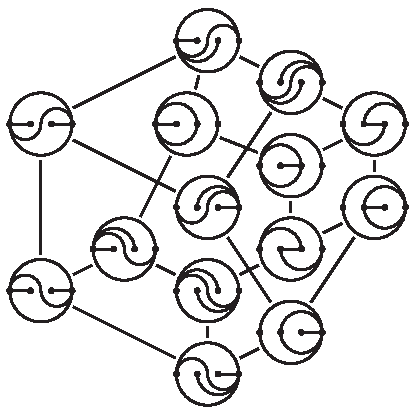
\includegraphics[scale=1.7]{wigglyFlipGraph} \quad \begin{tikzpicture}%
	[x={(0.681462cm, -0.327528cm)},
	y={(0.731633cm, 0.326817cm)},
	z={(-0.017949cm, 0.886519cm)},
	scale=.900000,
	back/.style={color=blue, thin},
	edge/.style={color=blue, very thick, },
	facet/.style={fill=blue,fill opacity=0.00000},
	vertex/.style={inner sep=1pt,circle,draw=blue,fill=blue,thick}]
%
%
%% This TikZ-picture was produce with Sagemath version 9.5
%% with the command: ._tikz_3d_in_3d and parameters:
%% view = [-764, -346, -545]
%% angle = 76.39
%% scale = 1
%% edge_color = blue
%% facet_color = blue
%% opacity = 0.5
%% vertex_color = blue
%% axis = False

%% Coordinate of the vertices:
%%
\coordinate (-1.00000, -4.00000, -3.00000) at (-1.00000, -4.00000, -3.00000);
\coordinate (1.00000, 0.00000, -3.00000) at (1.00000, 0.00000, -3.00000);
\coordinate (3.00000, 4.00000, 1.00000) at (3.00000, 4.00000, 1.00000);
\coordinate (3.00000, 2.00000, -1.00000) at (3.00000, 2.00000, -1.00000);
\coordinate (3.00000, 0.00000, -1.00000) at (3.00000, 0.00000, -1.00000);
\coordinate (1.00000, -2.00000, -3.00000) at (1.00000, -2.00000, -3.00000);
\coordinate (3.00000, 4.00000, 5.00000) at (3.00000, 4.00000, 5.00000);
\coordinate (3.00000, 0.00000, 3.00000) at (3.00000, 0.00000, 3.00000);
\coordinate (-1.00000, -4.00000, 1.00000) at (-1.00000, -4.00000, 1.00000);
\coordinate (-5.00000, -4.00000, 1.00000) at (-5.00000, -4.00000, 1.00000);
\coordinate (-5.00000, -4.00000, -3.00000) at (-5.00000, -4.00000, -3.00000);
\coordinate (-3.00000, 0.00000, -3.00000) at (-3.00000, 0.00000, -3.00000);
\coordinate (-1.00000, 4.00000, 1.00000) at (-1.00000, 4.00000, 1.00000);
\coordinate (-1.00000, 4.00000, 5.00000) at (-1.00000, 4.00000, 5.00000);
%%
%%
%% Drawing edges in the back
%%
\draw[edge,back] (1.00000, 0.00000, -3.00000) -- (-3.00000, 0.00000, -3.00000);
\draw[edge,back] (3.00000, 4.00000, 1.00000) -- (-1.00000, 4.00000, 1.00000);
\draw[edge,back] (-5.00000, -4.00000, -3.00000) -- (-3.00000, 0.00000, -3.00000);
\draw[edge,back] (-3.00000, 0.00000, -3.00000) -- (-1.00000, 4.00000, 1.00000);
\draw[edge,back] (-1.00000, 4.00000, 1.00000) -- (-1.00000, 4.00000, 5.00000);
%%
%%
%% Drawing vertices in the back
%%
\node[vertex] at (-1.00000, 4.00000, 1.00000)     {};
\node[vertex] at (-3.00000, 0.00000, -3.00000)     {};
%%
%%
%% Drawing the facets
%%
\fill[facet] (3.00000, 0.00000, 3.00000) -- (3.00000, 0.00000, -1.00000) -- (3.00000, 2.00000, -1.00000) -- (3.00000, 4.00000, 1.00000) -- (3.00000, 4.00000, 5.00000) -- cycle {};
\fill[facet] (1.00000, -2.00000, -3.00000) -- (1.00000, 0.00000, -3.00000) -- (3.00000, 2.00000, -1.00000) -- (3.00000, 0.00000, -1.00000) -- cycle {};
\fill[facet] (-1.00000, -4.00000, 1.00000) -- (-1.00000, -4.00000, -3.00000) -- (1.00000, -2.00000, -3.00000) -- (3.00000, 0.00000, -1.00000) -- (3.00000, 0.00000, 3.00000) -- cycle {};
\fill[facet] (-1.00000, 4.00000, 5.00000) -- (3.00000, 4.00000, 5.00000) -- (3.00000, 0.00000, 3.00000) -- (-1.00000, -4.00000, 1.00000) -- (-5.00000, -4.00000, 1.00000) -- cycle {};
\fill[facet] (-5.00000, -4.00000, -3.00000) -- (-1.00000, -4.00000, -3.00000) -- (-1.00000, -4.00000, 1.00000) -- (-5.00000, -4.00000, 1.00000) -- cycle {};
%%
%%
%% Drawing edges in the front
%%
\draw[edge] (-1.00000, -4.00000, -3.00000) -- (1.00000, -2.00000, -3.00000);
\draw[edge] (-1.00000, -4.00000, -3.00000) -- (-1.00000, -4.00000, 1.00000);
\draw[edge] (-1.00000, -4.00000, -3.00000) -- (-5.00000, -4.00000, -3.00000);
\draw[edge] (1.00000, 0.00000, -3.00000) -- (3.00000, 2.00000, -1.00000);
\draw[edge] (1.00000, 0.00000, -3.00000) -- (1.00000, -2.00000, -3.00000);
\draw[edge] (3.00000, 4.00000, 1.00000) -- (3.00000, 2.00000, -1.00000);
\draw[edge] (3.00000, 4.00000, 1.00000) -- (3.00000, 4.00000, 5.00000);
\draw[edge] (3.00000, 2.00000, -1.00000) -- (3.00000, 0.00000, -1.00000);
\draw[edge] (3.00000, 0.00000, -1.00000) -- (1.00000, -2.00000, -3.00000);
\draw[edge] (3.00000, 0.00000, -1.00000) -- (3.00000, 0.00000, 3.00000);
\draw[edge] (3.00000, 4.00000, 5.00000) -- (3.00000, 0.00000, 3.00000);
\draw[edge] (3.00000, 4.00000, 5.00000) -- (-1.00000, 4.00000, 5.00000);
\draw[edge] (3.00000, 0.00000, 3.00000) -- (-1.00000, -4.00000, 1.00000);
\draw[edge] (-1.00000, -4.00000, 1.00000) -- (-5.00000, -4.00000, 1.00000);
\draw[edge] (-5.00000, -4.00000, 1.00000) -- (-5.00000, -4.00000, -3.00000);
\draw[edge] (-5.00000, -4.00000, 1.00000) -- (-1.00000, 4.00000, 5.00000);
%%
%%
%% Drawing the vertices in the front
%%
\node[vertex] at (-1.00000, -4.00000, -3.00000)     {};
\node[vertex] at (1.00000, 0.00000, -3.00000)     {};
\node[vertex] at (3.00000, 4.00000, 1.00000)     {};
\node[vertex] at (3.00000, 2.00000, -1.00000)     {};
\node[vertex] at (3.00000, 0.00000, -1.00000)     {};
\node[vertex] at (1.00000, -2.00000, -3.00000)     {};
\node[vertex] at (3.00000, 4.00000, 5.00000)     {};
\node[vertex] at (3.00000, 0.00000, 3.00000)     {};
\node[vertex] at (-1.00000, -4.00000, 1.00000)     {};
\node[vertex] at (-5.00000, -4.00000, 1.00000)     {};
\node[vertex] at (-5.00000, -4.00000, -3.00000)     {};
\node[vertex] at (-1.00000, 4.00000, 5.00000)     {};
%%
%%
\end{tikzpicture}}

\end{slide}

%%%%%%%%%%%%%%%%%%%%%%%%%%%%%%%%%%%%%%%%%%%%%%%%%%%%%%

\partie{Cambrian considerations}

%%%%%%%%%%%%%%%%%%%%%%%%%%%%%%%%%%%%%%%%%%%%%%%%%%%%%%

\begin{slide}{Cambrian considerations}

\theo{THM}{
For $\delta = \delta_1 \dots \delta_n \in \{+,-\}^n$, there are lattice isomorphisms between 

\vspace{-.4cm}
\begin{itemize}
\item \emph{$\delta$-triangulations} $=$ triangulation of the $\delta$-gon, whose vertex at abscissa $i$ has ordinate \\[-1cm]
\[
\text{positive if $\delta_j = {+}$
\qquad and \qquad
negative if $\delta_j = {-}$}
\]
\vspace{-1.5cm}
\item \emph{$\delta$-permutations} $=$ permutation of~$[n]$ avoiding for~$i < j < k$ \\[-1cm]
\[
\cdots j \cdots ki \cdots \text{ if~$\delta_j = +$}
\quad\text{and}\quad
\cdots ik \cdots j \cdots \text{ if~$\delta_j = -$}
\]
\vspace{-1.5cm}
\item \emph{$\delta$-wiggly pseudotriangulations} $=$ wiggly pseudotriangulation containing the arcs \\[-1cm]
\[
(0, j, {[1,j[}, \varnothing) \text{ for~$\delta_j = {+}$}
\qquad\text{and}\qquad
(0, j, \varnothing, {[1,j[}) \text{ for~$\delta_j = {-}$}
\]
\vspace{-1.5cm}
\item \emph{$\delta$-wiggly permutations} $=$ wiggly permutation~$\sigma$ of~$[2n]$ such that \\[-1cm]
\[
\delta_j = {+} \quad \Longrightarrow \quad \sigma^{-1}(i) \le \sigma^{-1}(2j-1)
\quad\text{and}\quad
\delta_j = {-} \quad \Longrightarrow \quad \sigma^{-1}(2j) \le \sigma^{-1}(i)\quad\;\;
\]
\end{itemize}

\vspace{-.5cm}
\hfill \papier{Bapat--P. (24$^+$)}

}

\vspace{.3cm}
\centerline{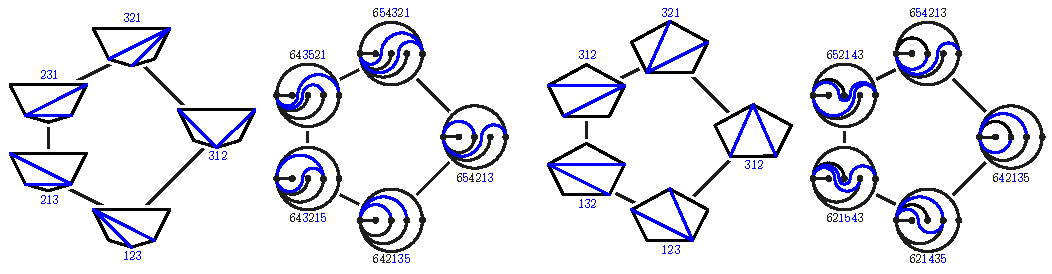
\includegraphics[scale=1.6]{wigglyCambrian1}}

\end{slide}

%%%

\begin{slide}{Cambrian considerations}

\theo{THM}{
For $\delta = \delta_1 \dots \delta_n \in \{+,-\}^n$, there are lattice isomorphisms between 
\begin{compactitem}
\item $\delta$-triangulations
\item $\delta$-permutations
\item $\delta$-wiggly pseudotriangulations
\item $\delta$-wiggly permutations \hfill \papier{Bapat--P. (24$^+$)}
\end{compactitem}
}

\vspace{.5cm}
\centerline{\includegraphics[scale=1.5]{wigglyCambrian2}}

\end{slide}

%%%

\begin{slide}{Cambrian considerations}

\theo{THM}{
For $\delta = \delta_1 \dots \delta_n \in \{+,-\}^n$, there are lattice isomorphisms between 
\begin{compactitem}
\item $\delta$-triangulations
\item $\delta$-permutations
\item $\delta$-wiggly pseudotriangulations
\item $\delta$-wiggly permutations \hfill \papier{Bapat--P. (24$^+$)}
\end{compactitem}
}

\vspace{-.2cm}
\centerline{\includegraphics[scale=1.5]{wigglyCambrian3}}

\end{slide}

%%%

\begin{slide}{Cambrian considerations}

\theo{THM}{
For $\delta = \delta_1 \dots \delta_n \in \{+,-\}^n$, there are lattice isomorphisms between 
\begin{compactitem}
\item $\delta$-triangulations
\item $\delta$-permutations
\item $\delta$-wiggly pseudotriangulations
\item $\delta$-wiggly permutations \hfill \papier{Bapat--P. (24$^+$)}
\end{compactitem}
}

\vspace{.5cm}
\theo{PROP}{
The $\delta$-associahedron~$\Asso_\delta$ is normally equivalent to the face of the wigglyhedron~$\wigglyhedron_n$ corresponding to the wiggly pseudodissection formed by the $\delta$-wiggly arcs.

\hfill \papier{Bapat--P. (24$^+$)}

}

\end{slide}

%%%%%%%%%%%%%%%%%%%%%%%%%%%%%%%%%%%%%%%%%%%%%%%%%%%%%%

\partie{Some open problems}

%%%%%%%%%%%%%%%%%%%%%%%%%%%%%%%%%%%%%%%%%%%%%%%%%%%%%%

\begin{slide}{Open problem 1: graph properties of wigglyhedron}

\centerline{\includegraphics[scale=1.7]{wigglyFlipGraph}\quad\includegraphics[scale=1.7]{wigglyLattice}}

\theo{Q1a}{Is the wiggly flip graph Hamiltonian?

\hfill \color{gray}{[NB: wiggly permutations do not form a zigzag language]}
}

\theo{Q1b}{What is the diameter of the wiggly flip graph?

%\hfill \color{gray}{[NB: $2n-1 \le \delta_n$]}
}

\end{slide}

%%%%%%%%%%%%%%%%%%%%%%%%%%%%%%%%%%%%%%%%%%%%%%%%%%%%%%

\begin{slide}{Open problem 2: wiggly pseudotriangulations and duality}
%\hspace{1.6cm} triangulations \hspace{3.4cm} pseudotriangulations \hspace{2.5cm} multitriangulations\\
%\vspace{-.5cm}\\

\vspace*{-.8cm}
\hspace*{-.6cm}\includegraphics[scale=1.9]{geometricStructures7}
\vspace{-10.5cm} \\ \hspace*{25.7cm} ${k=2}$

\vspace{7.8cm}
\theo{Q2}{Is there a dual interpretation of wiggly pseudotriangulations?}

\vspace*{-3cm}
\end{slide}

%%%%%%%%%%%%%%%%%%%%%%%%%%%%%%%%%%%%%%%%%%%%%%%%%%%%%%

\begin{slide}{Open problem 3: wiggly pseudotriangulations of point sets}

$\b{P}$ arbitrary point set in the plane

\emph{wiggly complex}~$\wigglyComplex_{\b{P}}$ = simplicial complex of non-crossing and pointed wiggly edges

\vspace{-.5cm}\hspace{14.5cm}
\rotatebox{270}{\includegraphics[scale=1.1]{wigglyComplexSquare}}

\vspace*{-15cm}
\begin{minipage}{13cm}
\theo{Q3a}{Is~$\wigglyComplex_{\b{P}}$ the boundary complex of a simplicial polytope?

\color{gray}{
[NB: aligned points $\Rightarrow$ wigglyhedron \\
general position $\Rightarrow$ Rote--Santos--Streinu]
}

\vspace{.1cm}
}

\vspace{1cm}
\theo{Q3b}{Is the graph of~$\wigglyComplex_{\b{P}}$ Hamiltonian?}

\end{minipage}

\end{slide}


%%%%%%%%%%%%%%%%%%%%%%%%%%%%%%%%%%%%%%%%%%%%%%%%%%%%%%

\newpage

\vspace*{2cm}
\centerline{\includegraphics[scale=1.8]{wigglyFlipGraph}\quad\raisebox{.5cm}{\includegraphics[scale=1.8]{wigglyLattice}}}

\vspace*{.2cm}
\centerline{\includegraphics[scale=4]{wigglyThankYou}}

\end{document}

